\section{Monday for MAT4002}\index{Monday_lecture}

\subsection{Introduction to Topology}
We will study global properties of a geometric object, i.e., \textit{the distrance between 2 points in an object is totally ignored}. For example, the objects shown below are essentially invariant under a certain kind of transformation:
\begin{figure}[H]
\centering

\includegraphics[width=5cm]{week1/f_2_1}

\includegraphics[width=5cm]{week1/f_2_2}
\end{figure}
Another example is that the coffee cup and the donut have the same topology:
 \begin{figure}[H]
\centering
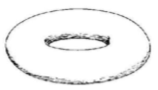
\includegraphics[width=5cm]{week1/f_2_3}
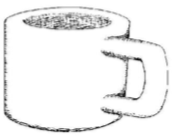
\includegraphics[width=5cm]{week1/f_2_4}
\end{figure}
However, the two objects below have the intrinsically different topologies:
 \begin{figure}[H]
\centering

\includegraphics[width=5cm]{week1/f_2_5}
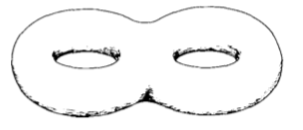
\includegraphics[width=5cm]{week1/f_2_6}
\end{figure}
In this course, we will study the phenomenon described above mathematically.

\subsection{Metric Spaces}
In order to ingnore about the distances, we need to learn about distances first.
\begin{definition}[Metric Space]
Metric space is a set $X$ where one can measure distance between any two objects in X.

Specifically speaking, a metric space $X$ is a non-empty set endowed with a function (distance function) $d:X\times X\to\mathbb{R}$ such that
\begin{enumerate}
\item
$d(\bm x,\bm y)\ge0$ for $\forall\bm x,\bm y\in X$ with equality iff $\bm x=\bm y$
\item
$d(\bm x,\bm y)=d(\bm y,\bm x)$
\item
$d(\bm x,\bm z)\le d(\bm x,\bm y)+d(\bm y,\bm z)$ (triangular inequality)
\end{enumerate}
\end{definition}

\begin{example}
\begin{enumerate}
\item
Let $X=\mathbb{R}^n$, with 
\[
d_2(\bm x,\bm y)=\sqrt{\sum_{i=1}^n(x_i-y_i)^2}
\]
\[
d_\infty(\bm x,\bm y)=\max_{i=1,\dots,n}|x_i-y_i|
\]
\item
Let $X$ be any set, and define the discrete metric 
\[
d(\bm x,\bm y)=\left\{
\begin{aligned}
0,&\quad\mbox{if }x=y\\
1,&\quad\mbox{if }x\ne y
\end{aligned}
\right.
\]
\end{enumerate}
Homework: Show that (1) and (2) defines a metric.
\end{example}
\begin{definition}[Open Ball]
An \emph{open ball} of radius $r$ centered at $\bm x\in X$ is the set
\[
B_r(\bm x)=\{\bm y\in X\mid d(\bm x,\bm y)<r\}
\]
\end{definition}
\begin{example}
\begin{enumerate}
\item
The set $B_1(0,0)$ defines an open ball under the metric $(X=\mathbb{R}^2,d_2)$, or the metric $(X=\mathbb{R}^2,d_\infty)$. The corresponding diagram is shown below:
 \begin{figure}[H]
\centering
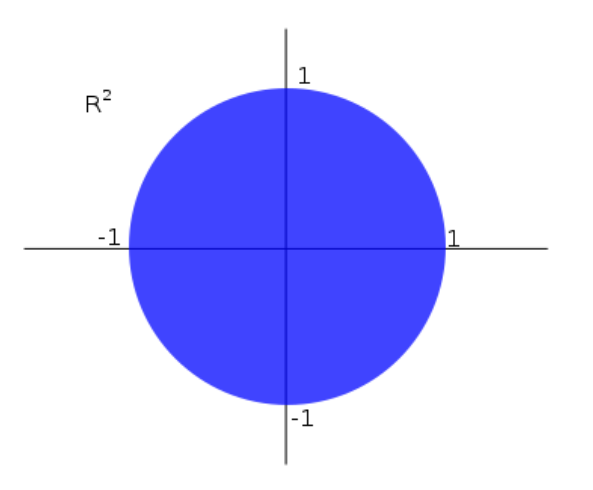
\includegraphics[width=5cm]{week1/f_1_2}
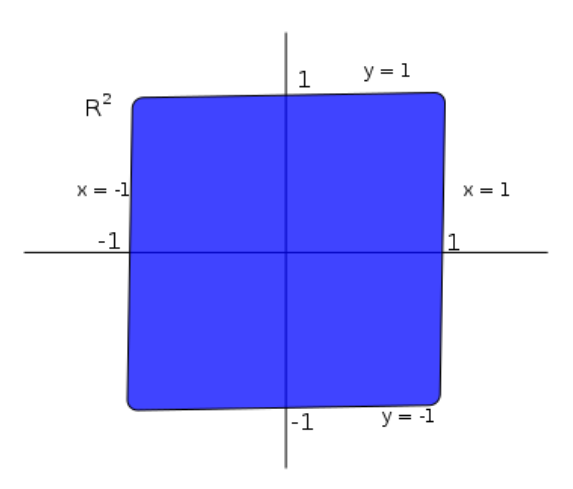
\includegraphics[width=5cm]{week1/f_1_3}
\caption{Left: under the metric $(X=\mathbb{R}^2,d_2)$; Right: under the metric $(X=\mathbb{R}^2,d_\infty)$}
\end{figure}
\item
Under the metric $(X=\mathbb{R}^2,\text{discrete metric})$, the set $B_1(0,0)$ is one single point, also defines an open ball.
\end{enumerate}
\end{example}

\begin{definition}[Open Set]
Let $X$ be a metric space, $U\subseteq X$ is an open set in $X$ if $\forall u\in U$, there exists $\epsilon_u>0$ such that $B_{\epsilon_u}(u)\subseteq U$.
\end{definition}
\begin{definition}
The \emph{topology} induced from $(X,d)$ is the collection of all open sets in $(X,d)$, denoted as the symbol $\mathcal{T}$.
\end{definition}
\begin{proposition}
All open balls $B_r(\bm x)$ are open in $(X,d)$.
\end{proposition}
\begin{proof}
Consider the example $X=\mathbb{R}$ with metric $d_2$. Therefore $B_r(x)=(x-r,x+r)$. Take $\bm y\in B_r(\bm x)$ such that $d(\bm x,\bm y)=q<r$ and consider $B_{(r-q)/2}(\bm y)$: for all $z\in B_{(r-q)/2}(\bm y)$, we have
\[
d(\bm x,\bm z)\le d(\bm x,\bm y)+d(\bm y,\bm z)<q+\frac{r-q}{2}<r,
\]
which implies $\bm z\in B_r(x)$.
\end{proof}

\begin{proposition}\label{Pro:1:6}
Let $(X,\bm d)$ be a metric space, and $\mathcal{T}$ is the topology induced from $(X,d)$, then
\begin{enumerate}
\item
let the set $\{G_\alpha\mid\alpha\in\mathcal{A}\}$ be a collection of (uncountable) open sets, i.e., $G_\alpha\in\mathcal{T}$, then $\bigcup_{\alpha\in\mathcal{A}}G_\alpha\in\mathcal{T}$.
\item
let $G_1,\dots,G_n\in\mathcal{T}$, then $\bigcap_{i=1}^nG_i\in\mathcal{T}$. The finite intersection of open sets is open.
\end{enumerate}
\end{proposition}
\begin{proof}
\begin{enumerate}
\item
Take $x\in\bigcup_{\alpha\in\mathcal{A}}G_\alpha$, 
then $x\in G_\beta$ for some $\beta\in\mathcal{A}$. 
Since $G_\beta$ is open, there exists $\epsilon_x>0$ s.t.
\[
B_{\epsilon_x}(x)\subseteq G_\beta\subseteq\bigcup_{\alpha\in\mathcal{A}}G_\alpha
\]
\item
Take $x\in\bigcap_{i=1}^nG_i$, i.e., $x\in G_i$ for $i=1,\dots,n$, i.e., there exists $\epsilon_i>0$ such that $B_{\epsilon_i}(x)\subseteq G_i$ for $i=1,\dots,n$. Take $\epsilon=\min\{\epsilon_1,\dots,\epsilon_n\}$, which implies
\[
B_\epsilon(x)\subseteq B_{\epsilon_i}(x)\subseteq G_i,\forall i
\]
which implies $B_\epsilon(x)\subseteq\bigcap_{i=1}^nG_i$
\end{enumerate}
\end{proof}
\paragraph{Exercise}
\begin{enumerate}
\item
let $\mathcal{T}_2,\mathcal{T}_\infty$ be topologies induced from the metrices $d_2,d_\infty$ in $\mathbb{R}^2$. Show that $J_2=J_\infty$, i.e., every open set in $(\mathbb{R}^2,d_2)$ is open in $(\mathbb{R}^2,d_\infty)$, and every open set in $(\mathbb{R}^2,d_\infty)$ is open in $(\mathbb{R}_2,d_2)$.






\item
Let $\mathcal{T}$ be the topology induced from the discrete metric $(X,d_{\text{discrete}}).$ What is $\mathcal{T}$?

\end{enumerate}












